
\section{Augmented Reality}

Augmented Reality (AR) ist eine Klasse aus dem Realitäts-Virtualitäts-Kontinuum von \cite{milgram1995augmented}, welches in Abbildung \ref{fig:virtual-continuum} abgebildet ist. Diese Klasse beschreibt die Darstellungen von realen und virtuellen Informationen in einer Repräsentationsform, wobei hier reale und virtuelle Objekte in einer realen Umgebung kombiniert dargestellt werden können. Diese virtuellen Objekte sind in der realen Umgebung idealerweise fest lokalisiert und fügen sich somit in das reale Erscheinungsbild ein. Typischerweise sind AR Anwendungen interaktiv, und stellen die virtuellen Objekte in Echtzeit und dreidimensional in der realen Welt dar. Für die Definition von AR Anwendungen gibt es zudem keine Limitierung für die Darstellungstechnologie, wie zum Beispiel das Projekt Tango Tablett oder einem Head-Mounted Display. AR beschränkt sich zudem nicht auf den angesprochenen Sinn - so sind zum Beispiel AR Anwendungen mit visueller, taktiler oder sogar olfaktorischer Umsetzung möglich.\\

\begin{figure}
  \centering
	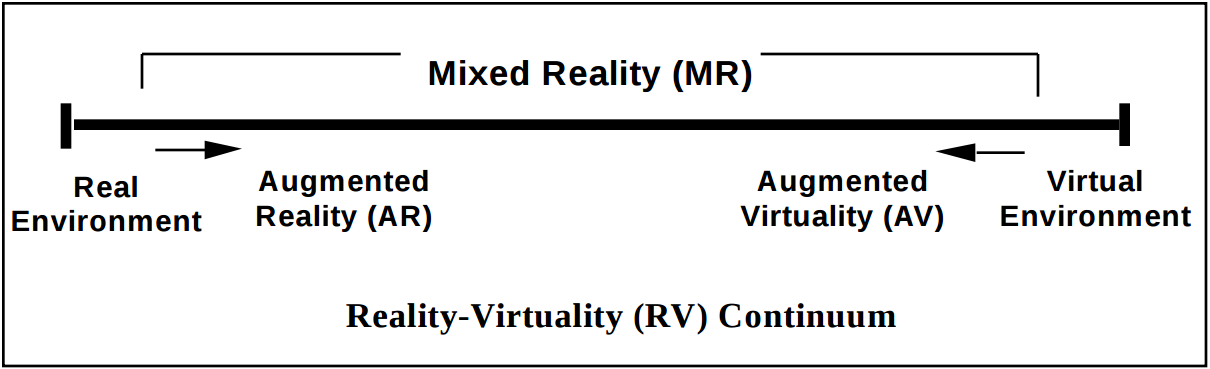
\includegraphics[width=0.85\textwidth]{content/images/theory/virtual-continuum.png} 
  \caption{Vereinfachte Darstellung des Realitäts-Virtualitäts-Kontinuum von \citet*{milgram1995augmented}}
  \label{fig:virtual-continuum}
\end{figure}


Virtuel Reality (VR) oder auch Virtual Environment hingegen kapselt sich von der realen Umgebung ab und bietet Interaktionen in reinen virtuellen Umgebungen. Diese rein virtuelle Darstellung konnte sich im Gegensatz zu Augmented Reality deutlich schneller Entwickeln, da die technologischen Anforderungen an AR deutlich höher sind. \citep{van2010survey}\\

\subsection{Technische Anforderungen}

Dieser Abschnitt widmet sich den technischen Anforderungen an Augmented Reality, indem die potentiellen Display Technologien beschrieben werden, mögliche Trackingverfahren zur Ermittlung der Betrachtungsposition erläutern werden und auch die Systeme behandelt werden, mit denen ein Nutzer mit den virtuellen Darstellungen interagieren kann.\\

\subsubsection{Display Technologie}

Der erste wichtige Teil der technologischen Anforderungen an AR sind visuelle Anzeigen (visual displays), die neben der Möglichkeit eines dreidimensionalen Renderings, welches hier aus der Virtual Reality vorausgesetzt werden soll, weitere Charakteristika mit sich bringen. Nach \citet{van2010survey} lassen sich diese Technologien zunächst in je drei Arten der Darstellung und Positionierung unterteilen.  \\

Die einfachste und günstigste Art der visuellen Darstellung in AR ist \enquote{video see-through}, wodurch die reale Umgebung durch eine Video Aufnahme ersetzt wird und die virtuellen Objekte digital in die Video Aufnahme gerendert werden. Das bietet die Möglichkeit Objekte aus der realen Umgebung zu entfernen oder zu ändern oder, anhand der Luminanz Information vom Video, das Rendering der virtuellen Objekte entsprechend an die Realität anzupassen. Anwendung findet diese Technologie typischerweise in Tablets oder Smartphones.\\

Die nächste Möglichkeit zur Darstellung ist \enquote{optical see-through}. Hier werden die virtuellen Objekte durch transparente Spiegel in das Sichtfeld des Betrachters gebracht. Anders als bei \enquote{video see-throught} bleibt die reale Auflösung für die visuelle Aufnahme des Betrachtes gleich und es können zudem keine Latenzprobleme beim Ändern des Betrachtungswinkels auftreten (parallax-effect). Auf der anderen Seite besteht bei dieser Technologie das Problem, dass die Darstellung von virtuellen Objekten nicht kräftig genug ist, um die reale Umgebung auf Grund von der transparenten Darstellungsoberfläche komplett auszublenden. Typische Geräte dieser Technologie sind Headmounted Displays wie Google Glass oder stationäre Geräte wie der HoloDesk.\\

Die dritte Möglichkeit ist die projizierte Darstellung, in der die Augmented Reality Überlagerung auf die realen Objekte projiziert werden. Diese Darstellung ermöglicht die Abdeckung vom gesamten Sichtfeld des Betrachters, benötigt aber eine entsprechende Kalibrierung oder eine Strukturwahrnehmung bei Umgebungsänderungen.\\

Neben der Art der Darstellung können die Display Technologien laut \citet{azuma2001recent} anhand Ihrer Positionierung klassifiziert werden. Man unterscheidet zwischen am Kopf befestigten Displays (head-mounted), tragbaren Displays (hand-held) und räumlich positionierten Displays. Zu jeder dieser Displayarten gibt es wiederum unterschiedliche technische Umsetzungen mit ihren spezifischen Vor- und Nachteilen bezüglich ihrer Anwendungsszenarien.\\

\subsubsection{Tracking Technologien}

Um eine virtuelle Projektion im realen Raum auf nicht stationären Displaytechnologien zu realisieren muss die Position und gegebenenfalls relative Positionsänderung des Displays bestimmt werden, auch \enquote{augmented reality registration} genannt. Man spricht dabei üblichweise von den \enquote{six degrees of freedom (6DOF)}, der Position im Raum (x, y, z) und der Orientierung (yaw, pitch, roll). \\

Frühe Techniken für die Registrierung benötigten üblicher Weise eine speziell vorbereitete Räumlichkeit, denn sie basierten auf mechanischen, magnetischen oder Ultraschall Sensoren um die Position zu bestimmen. Diese Sensoren sind zwar immer noch im Einsatz und bilden auch den Grundstein für die AR und VR Forschung, sind aber praktisch gesehen zu komplex und aufwändig für die meisten Anwendungsfälle. \citep{van2010survey} \\

Für ein grobes Positions-Tracking, vor allem auch außerhalb von Gebäuden wird GPS genutzt. Für großräumliche Anwendung ist GPS, mit einer Varianz von 10-15 Metern und in Kombination mit einem Kompass, durchaus praktikabel. Zum Beispiel um sichtbare Flugzeuge oder Sterne visuell aufzubereiten. Innerhalb von Gebäuden basiert die grobe Positionierung laut \citet{van2010survey} oft auf verfügbaren Wifi Access Points oder RFID Markern. \citet{lamarca2005place} demonstrieren hierzu auch die Möglichkeit diese Idee für grobe Lokalisation außerhalb von Gebäuden einzusetzen.\\

Optische Tracking Verfahren basierend auf Bildverarbeitung bieten laut \citet{van2010survey} deutlich genauere Resultate als die zuvor beschriebenen Verfahren. Es gibt hier viele verschiedene sensorische Ansätze ein optisches Tracking zu realisieren. Frühe verfahren nutzten referenzielle Marker oder Licht emittierende LEDs in einem vordefinierten Modell, um zwischen aufgenommenen Bildern eine homographische Transformation zu berechnen und um somit Rückschlüsse auf die Rotation und Positionsänderung der Kamera zu ziehen. Neue Verfahren ohne Marker, wie das sogenannte \enquote{visual odometry} von \citet{nister2004visual}, nutzen Techniken zur Feature Detection und Matching um Referenzen und Bewegungen zwischen aufgenommenen Bildern zu bestimmen.\\

Viele kommerzielle und erfolgreiche Tracking Verfahren beruhen jedoch auf hybride Ansätze, in denen die Informationen mehrerer Sensoren kombiniert werden, um potentielle Messfehler eines Sensors oder einer Methodik auszuschließen. So werden zum Beispiel Neigungssensor, Kompass und Gyroskop mit einem optischen Verfahren kombiniert, um ein Tracking der sechs Freiheitsgrade zu optimieren. Diese Erweiterung des optischen Verfahrens wird auch \enquote{visual-inertial odometry} genannt. \citep{van2010survey}\\

\citet{azuma2001recent} erwähnt an dieser Stelle auch die Kalibrierung der Sensoren, die für ein präzises Registrieren nötig ist. So müssen zum Beispiel die Linseneigenschaften der Kamera für optisches Tracking bekannt sein, damit die Verfahren mit Krümmungen, Verzerrungen und den perspektivischen Eigenschaften umgehen können. Diese Informationen sind auch bei video see-through Displays für ein korrektes Projizieren der 3D Objekte wichtig. Zudem wird erwähnt, dass man Messfehlern oder Drifts der Position zum Beispiel mit der Zunahme von Gyroscop Informationen entgegenwirken kann, indem man Ereignisse wie einen Schritt des Nutzers einfließen lässt. \citep{azuma2001recent} \\

\subsubsection{Interaktions Technologien} \label{sec:ar-interaction}

Neben den Display und Tracking Technologien ist es notwendig dem Nutzer andere Interaktionsmöglichkeiten anzubieten, da in der Regel das klassische zweidimensionale WIMP Paradigma (Windows, Icons, Menus and Pointer) im dreidimensionalen Kontext von AR keine ausreichende Gebrauchstauglichkeit bietet. Dennoch müssen die Interaktionstechnologien in Augmented Reality die üblichen Interaktionen wie aus WIMP unterstützen. Dazu gehören zum Beispiel das Auswählen, Positionieren und Drehen von virtuellen Objekten, das Zeichnen von Pfaden oder Flugbahnen, sowie die Eingabe von Quantitativen Werten oder Texten. \citep{van2010survey} \\

Frühe Augmented Realilty Systeme nutzen einfache Trackballs, Trackpads, Touchscreens oder Gyroscopmäuse für eine zweidimensionale Interaktion mit dem System. Später wurden dreidimensionale Equivalente eingeführt, wie 3D Mäuse oder Stifte, die eine dreidimensionale Interaktion ermöglichen. Diese Greifbaren Schnittstellen werden auch TUIs genannt (Tangible User Interface) und ermöglichen eine unidirektionale Interaktion mit dem System. Zudem wurden auch TUIs mit haptischen Feedback eingeführt, wie zum Beispiel die 3D Maus PHANTOM. \citep{van2010survey} \\

Eine weitere Art der TUIs sind laut \citet{azuma2001recent} Gegenstände, mit denen der Nutzer natürlich interagieren kann und die vom System optisch erfasst werden, um die Positionsänderung der Objekte anhand von Markern oder anderen optischen Merkmalen zu bestimmen. Somit kann ein Nutzer, zum Beispiel, für die virtuelle Einrichtung eines Raums, die Möbel mit Hilfe eines echten Gegenstands im Raum verschieben. \\

Nicht taktile Systeme verwenden meist optische Aufnahmen um Gesten der Hände, des gesamten Körpers oder die Blickrichtung des Nutzers zu erkennen. Dabei werden Kameras am Körper oder im Raum verwendet. Außerdem ist es Möglich Spracherkennung in die Interaktion mit einfließen zu lassen, um eine möglichst authentische Interaktion zu bieten. Wie auch bei den Tracking Technologien existieren hierbei Hybride Systeme, die verschiedene Interaktions Technologien kombinieren. \citep{van2010survey} \\

\subsection{Anwendungsbereiche}

Über die Jahre habe Wissenschaftler immer mehr Bereiche identifiziert, die von der Anwendung von Augmented Reality profitieren können. \citet{van2010survey} nennt dazu als Erstes Einsatzgebiet die persönliche Assistenz, in der AR Systeme eingesetzt werden können, um zum Beispiel mit Hilfe von Brillen (zum Beispiel der Google Glass) Namen der sichtbaren Personen anzuzeigen, die Navigation in unbekannten Regionen einzublenden oder beim Sightseeing Kontext relevante Informationen im Sichtfeld anzuzeigen. \\

Neben der persönlichen Assistenz können auch Anwendungen in der Industrie laut \citet{van2010survey} von AR profitieren. Es lassen sich zum Beispiel virtuelle Designumgebungen umsetzten, die es ermöglichen ein Auto in Lebensgröße zu Gestalten. Auch bei der Fertigung und Konstruktion können den Arbeitern unterstützende Informationen angezeigt werden. So werden zum Beispiel zu erledigende Schweißstellen hervorgehoben oder der Plan zur Konstruktion entsprechend eingeblendet. Oder für die Instandhaltung komplexer Maschinen kann ein AR System dem Nutzer eine Art Röntgenblick Hinweise auf potentielle Schwachstellen liefern. Auch in der Rüstungsindustrie existieren Anwendungsgebiete für Augmented Reality Systeme. So können zum Beispiel Gefechte für eine Kampfausbildung besser simuliert werden. \citep{azuma2001recent} \\

Für Anwendungsbereiche in der Medizin ist ein sehr genaues Tracking der Freiheitsgrade erforderlich, da AR in der Chirurgie und Behandlung von Patienten Anwendung findet. Erstellte Röntgenbilder oder Ultraschallbilder können hierdurch, anstatt auf einem separaten Monitor, direkt auf die entsprechende Körperstelle projiziert werden, wodurch gegebenenfalls eine genauere Untersuchung oder Behandlung möglich ist. \citep{van2010survey} \\

Augmented Reality wird auch im Entertainment Sektor eingesetzt. Videoübertragungen von Sportereignissen werden heutzutage oft durch zusätzliche Informationen angereichert. So erhalten zum Beispiel American Football Spiele dynamische Spielfeld Begrenzungen. Auch die Werbeeinblendungen am Rand des Spielfelds können entsprechend dem Gebiet der Ausstrahlung ausgetauscht werden. \citep{azuma2001recent} \\

Ein weiteres Großes Anwendungsgebiet für Augmented Reality sind laut \citet{azuma2001recent} Computerspiele, in denen es möglich ist in einer beliebigen Umgebung Objekte eines Spiels im Raum zu platzieren und mit Ihnen entsprechend zu interagieren. Die natürlichere Interaktion, gegenüber herkömmlichen Spielplattformen, und die Nutzung in einer persönlichen Spielumgebung führt zu einem intensiveren Spielerlebnis. \\

In der Bildung für Schulen oder Museen ist es auch mögliche AR Systeme einzusetzen. Zur Vermittlung von geometrischen oder mathematischen Grundlagen gibt es die Möglichkeit der kollaborativen und interaktiven Visualisierung von Körpern, an denen etwa Parameter manipuliert werden, um danach Ihre Eigenschaften zu beobachten. \citep{van2010survey} \\

\subsection{Einschränkungen und Probleme}

Die frühen Augmented Reality Systeme sind auf Grund ihrer Größe sehr unhandlich und mobil daher nur mit großem Aufwand anwendbar. Durch die Verfügbarkeit mobiler und performanter Endgeräte ist ein mobiler Einsatz wiederum ermöglicht worden. Jedoch besitzen die aktuellen Geräte wie Smartphones oder Tabletts nicht die entsprechende Sensorik für ein präzises Tracking der sechs Freiheitsgrade. \citet{van2010survey} weisen zudem darauf hin, dass die Registrierung der Tiefe für die Anwendung von Überdeckungen oder korrekter Positionierung bei einer Interaktion ein komplexes Problem sei. Wie in Kapitel \ref{sec:theory_project_tango} zu finden geht Project Tango dieses Problem der Sensorik entsprechend an und Versucht Schnittstellen zu bieten, um sowohl das Tracking zu ermöglichen und Tiefeninformationen über die aktuelle Szene zu liefern. \\

Eine weitere erwähnenswerte Problematik ist neben der sensorischen Themen von Augmented Reality die Herangehensweise zur Gestaltung der Nutzeroberflächen für AR. Denn die UI Konzeption gestaltet sich, laut \citet{azuma2001recent}, als schwierig. Die Anreicherungen durch Augmented Reality führt schnell dazu, dass das Sichtfeld überladen wirkt. Jedoch sollte dem Nutzer immer die Informationen zur Verfügung gestellt werden, die gegebenenfalls kontextsensitive und relevant sind. Diese Angesprochenen Faktoren führen aktuell gegenüber Augmented Reality noch zu einer geringen Akzeptanz der Endverbraucher\\

